\chapter{Data Containers}\label{introduction-to-python---lesson-1.5}

In this chapter the container types available in $\tt{python}$ are reviewed.

\section{Lists}\label{lists}

A list in $\tt{python}$ is a container that is a \emph{mutable}, ordered sequence of elements. Each element or value that is inside of a list is called an *item*. Each item can be accessed using square brackets notation (very important, list indexing is zero-based so the first element is the 0th). A list is considered mutable since you can add, remove or update the items in it. Ordered instead means that items are kept in the same order they have been added.
Lists can be created by enclosing in square brackets the comma-separated list of the items or using the $\tt{list()}$ operator.

\begin{tcolorbox}[breakable, size=fbox, boxrule=1pt, pad at break*=1mm, colback=cellbackground, colframe=cellborder]
\begin{Verbatim}[commandchars=\\\{\}]
\PY{n}{mylist} \PY{o}{=} \PY{p}{[}\PY{l+m+mi}{21}\PY{p}{,} \PY{l+m+mi}{32}\PY{p}{,} \PY{l+m+mi}{15}\PY{p}{]}
\PY{n+nb}{print}\PY{p}{(}\PY{n}{mylist}\PY{p}{)}
\PY{n+nb}{print} \PY{p}{(}\PY{n+nb}{type}\PY{p}{(}\PY{n}{mylist}\PY{p}{)}\PY{p}{)}

[21, 32, 15]
\end{Verbatim}
\end{tcolorbox}

\begin{tcolorbox}[breakable, size=fbox, boxrule=1pt, pad at break*=1mm, colback=cellbackground, colframe=cellborder]
\begin{Verbatim}[commandchars=\\\{\}]
\PY{n+nb}{print}\PY{p}{(}\PY{n}{mylist}\PY{p}{[}\PY{l+m+mi}{0}\PY{p}{]}\PY{p}{)}

21
\end{Verbatim}
\end{tcolorbox}

If you have a list of lists (i.e. a 2-dimensional list) you can use the square brackets multiple times to access the inner elements:
\begin{tcolorbox}[breakable, size=fbox, boxrule=1pt, pad at break*=1mm,colback=cellbackground, colframe=cellborder]
\begin{Verbatim}[commandchars=\\\{\}]                 
\PY{n}{alist} \PY{o}{=} \PY{p}{[}\PY{p}{[}\PY{l+m+mi}{1}\PY{p}{,}\PY{l+m+mi}{2}\PY{p}{]}\PY{p}{,} \PY{p}{[}\PY{l+m+mi}{3}\PY{p}{,}\PY{l+m+mi}{4}\PY{p}{]}\PY{p}{,} \PY{p}{[}\PY{l+m+mi}{5}\PY{p}{,}\PY{l+m+mi}{6}\PY{p}{]}\PY{p}{]}       
\PY{n+nb}{print} \PY{p}{(}\PY{n}{alist}\PY{p}{[}\PY{l+m+mi}{1}\PY{p}{]}\PY{p}{[}\PY{l+m+mi}{1}\PY{p}{]}\PY{p}{)} \PY{c+c1}{\PYZsh{} first [1] returns [3,4], second returns 4}                   
\end{Verbatim} 
\end{tcolorbox}  

The number of elements in a list is counted using the keyword \texttt{len()}:
\begin{tcolorbox}[breakable, size=fbox, boxrule=1pt, pad at break*=1mm, colback=cellbackground, colframe=cellborder]
\begin{Verbatim}[commandchars=\\\{\}]
\PY{n+nb}{print}\PY{p}{(}\PY{n+nb}{len}\PY{p}{(}\PY{n}{mylist}\PY{p}{)}\PY{p}{)}

3
\end{Verbatim}
\end{tcolorbox}

Looping on list items can be achieved in two ways: using directly the list or by index:

\begin{tcolorbox}[breakable, size=fbox, boxrule=1pt, pad at break*=1mm, colback=cellbackground, colframe=cellborder]
\begin{Verbatim}[commandchars=\\\{\}]
\PY{n+nb}{print} \PY{p}{(}\PY{l+s+s2}{\PYZdq{}}\PY{l+s+s2}{Loop using the list itself:}\PY{l+s+s2}{\PYZdq{}}\PY{p}{)}
\PY{k}{for} \PY{n}{i} \PY{o+ow}{in} \PY{n}{mylist}\PY{p}{:}
    \PY{n+nb}{print} \PY{p}{(}\PY{n}{i}\PY{p}{)}

\PY{n+nb}{print} \PY{p}{(}\PY{l+s+s2}{\PYZdq{}}\PY{l+s+s2}{Loop by index:}\PY{l+s+s2}{\PYZdq{}}\PY{p}{)}
\PY{k}{for} \PY{n}{i} \PY{o+ow}{in} \PY{n+nb}{range}\PY{p}{(}\PY{n+nb}{len}\PY{p}{(}\PY{n}{mylist}\PY{p}{)}\PY{p}{)}\PY{p}{:} \PY{c+c1}{\PYZsh{} len() returns the number of items in a list}
    \PY{n+nb}{print} \PY{p}{(}\PY{n}{mylist}\PY{p}{[}\PY{n}{i}\PY{p}{]}\PY{p}{)}

Loop using the list itself:
21
32
15

Loop by index:
21
32
15
\end{Verbatim}
\end{tcolorbox}

With the \texttt{enumerate} function is actually possible to do both at the same time since it returns two values, the index of the item and its value, so in the example below, \texttt{i} will take the item index values while \texttt{item} the item value itself:

\begin{tcolorbox}[breakable, size=fbox, boxrule=1pt, pad at break*=1mm, colback=cellbackground, colframe=cellborder]
\begin{Verbatim}[commandchars=\\\{\}]
\PY{k}{for} \PY{n}{i}\PY{p}{,} \PY{n}{item} \PY{o+ow}{in} \PY{n+nb}{enumerate}\PY{p}{(}\PY{n}{mylist}\PY{p}{)}\PY{p}{:}                        
    \PY{n+nb}{print} \PY{p}{(}\PY{n}{i}\PY{p}{,} \PY{n}{item}\PY{p}{)}

0 21
1 74
2 85
3 15
4 188
\end{Verbatim}
\end{tcolorbox}

Since a list is mutable we can dynamically change its items:

\begin{tcolorbox}[breakable, size=fbox, boxrule=1pt, pad at break*=1mm, colback=cellbackground, colframe=cellborder]
\begin{Verbatim}[commandchars=\\\{\}]
\PY{n}{mylist}\PY{p}{[}\PY{l+m+mi}{1}\PY{p}{]} \PY{o}{=} \PY{l+m+mi}{74} \PY{c+c1}{\PYZsh{} we can change list items since it\PYZsq{}s *mutable*}
\PY{n+nb}{print} \PY{p}{(}\PY{n}{mylist}\PY{p}{)}

[21, 74, 15]
\end{Verbatim}
\end{tcolorbox}

With \texttt{append} an item is added at the end, while with \texttt{insert} an item can be added in a specified position:

\begin{tcolorbox}[breakable, size=fbox, boxrule=1pt, pad at break*=1mm, colback=cellbackground, colframe=cellborder]
\begin{Verbatim}[commandchars=\\\{\}]
\PY{n}{mylist}\PY{o}{.}\PY{n}{append}\PY{p}{(}\PY{l+m+mi}{188}\PY{p}{)} \PY{c+c1}{\PYZsh{} append add an item at the end of the list}
\PY{n+nb}{print} \PY{p}{(}\PY{n}{mylist}\PY{p}{)}

[21, 74, 15, 188]
\end{Verbatim}
\end{tcolorbox}

To append multiple values at once to a list a loop can be used but \texttt{python} offers a single line way of doing it: \texttt{[i*2 for i in range(10)]}. This syntax is called \emph{list comprehension}.

\begin{tcolorbox}[breakable, size=fbox, boxrule=1pt, pad at break*=1mm, colback=cellbackground, colframe=cellborder]
\begin{Verbatim}[commandchars=\\\{\}]
\PY{n}{mylist}\PY{o}{.}\PY{n}{insert}\PY{p}{(}\PY{l+m+mi}{2}\PY{p}{,} \PY{l+m+mi}{85}\PY{p}{)} \PY{c+c1}{\PYZsh{} insert an item in the desired position }
                     \PY{c+c1}{\PYZsh{} (2 in this example)}
\PY{n+nb}{print} \PY{p}{(}\PY{n}{mylist}\PY{p}{)}

[21, 74, 85, 15, 188]
\end{Verbatim}
\end{tcolorbox}

Accessing items outside the list range gives an error:

\begin{tcolorbox}[breakable, size=fbox, boxrule=1pt, pad at break*=1mm, colback=cellbackground, colframe=cellborder]
\begin{Verbatim}[commandchars=\\\{\}]
\PY{n}{mylist}\PY{p}{[}\PY{l+m+mi}{10}\PY{p}{]} \PY{c+c1}{\PYZsh{} error ! it doesn\PYZsq{}t exists, the list has only 3 }
           \PY{c+c1}{\PYZsh{} elements, so the last is item 2}

---------------------------------------------------------------------------

IndexError                                Traceback (most recent call last)

<ipython-input-36-ed1e5e6c3e46> in <module>
----> 1 mylist[10] \# error ! it doesn't exists, the list has only 3
      2           \# elements, so the last is item 2

IndexError: list index out of range
\end{Verbatim}
\end{tcolorbox}

There are two more nice features of $\tt{python}$ indexing: negative
indices are like positive ones except that they starts from the last
element, and \emph{slicing} whcih allows to specify a range of indices.

\begin{tcolorbox}[breakable, size=fbox, boxrule=1pt, pad at break*=1mm, colback=cellbackground, colframe=cellborder]
\begin{Verbatim}[commandchars=\\\{\}]
\PY{n+nb}{print} \PY{p}{(}\PY{l+s+s2}{\PYZdq{}}\PY{l+s+s2}{negative index \PYZhy{}1 returns the last element:}\PY{l+s+s2}{\PYZdq{}}\PY{p}{,} \PY{n}{mylist}\PY{p}{[}\PY{o}{\PYZhy{}}\PY{l+m+mi}{1}\PY{p}{]}\PY{p}{)}
\PY{n+nb}{print} \PY{p}{(}\PY{l+s+s2}{\PYZdq{}}\PY{l+s+s2}{slice [1:3] returns items between the 1st and 2nd:}\PY{l+s+s2}{\PYZdq{}}\PY{p}{,} \PY{n}{mylist}\PY{p}{[}\PY{l+m+mi}{0}\PY{p}{:}\PY{l+m+mi}{3}\PY{p}{]}\PY{p}{)}
\PY{n+nb}{print} \PY{p}{(}\PY{l+s+s2}{\PYZdq{}}\PY{l+s+s2}{slice [:2] returns items between the 1st and 2nd:}\PY{l+s+s2}{\PYZdq{}}\PY{p}{,} \PY{n}{mylist}\PY{p}{[}\PY{p}{:}\PY{l+m+mi}{2}\PY{p}{]}\PY{p}{)}
\PY{n+nb}{print} \PY{p}{(}\PY{l+s+s2}{\PYZdq{}}\PY{l+s+s2}{slice [2:] returns items between the 2nd and the last:}\PY{l+s+s2}{\PYZdq{}}\PY{p}{,} \PY{n}{mylist}\PY{p}{[}\PY{l+m+mi}{2}\PY{p}{:}\PY{p}{]}\PY{p}{)}

negative index -1 returns the last element: 188
slice [1:3] returns items between the 1st and 2nd: [21, 74, 85]
slice [:2] returns items between the 1st and 2nd: [21, 74]
slice [2:] returns items between the 2nd and the last: [85, 15, 188]
\end{Verbatim}
\end{tcolorbox}

It is worth mentioning that a list doesn't have to be populated
with the same kind of objects (list indices are instead always
integers).

\begin{tcolorbox}[breakable, size=fbox, boxrule=1pt, pad at break*=1mm, colback=cellbackground, colframe=cellborder]
\begin{Verbatim}[commandchars=\\\{\}]
\PY{n}{mixedlist} \PY{o}{=} \PY{p}{[}\PY{l+m+mi}{1}\PY{p}{,} \PY{l+m+mi}{2}\PY{p}{,} \PY{l+s+s2}{\PYZdq{}}\PY{l+s+s2}{b}\PY{l+s+s2}{\PYZdq{}}\PY{p}{,} \PY{n}{math}\PY{o}{.}\PY{n}{sqrt}\PY{p}{]}
\PY{n+nb}{print} \PY{p}{(}\PY{n}{mixedlist}\PY{p}{)}

[1, 2, 'b', <built-in function sqrt>]
\end{Verbatim}
\end{tcolorbox}

\begin{tcolorbox}[breakable, size=fbox, boxrule=1pt, pad at break*=1mm, colback=cellbackground, colframe=cellborder]
\begin{Verbatim}[commandchars=\\\{\}]
\PY{n+nb}{print} \PY{p}{(}\PY{n}{mixedlist}\PY{p}{[}\PY{l+s+s1}{\PYZsq{}}\PY{l+s+s1}{k}\PY{l+s+s1}{\PYZsq{}}\PY{p}{]}\PY{p}{)}

---------------------------------------------------------------------------

TypeError                                 Traceback (most recent call last)

<ipython-input-72-aea4c7f9789e> in <module>()
----> 1 print (mixedlist['k'])
    
TypeError: list indices must be integers or slices, not str
\end{Verbatim}
\end{tcolorbox}

A complete list of the commands available for a list can be shown with the $\tt{dir}$ statement:

\begin{tcolorbox}[breakable, size=fbox, boxrule=1pt, pad at break*=1mm,colback=cellbackground, colframe=cellborder]
\begin{Verbatim}[commandchars=\\\{\}]
\PY{n+nb}{dir}\PY{p}{(}\PY{n+nb}{list}\PY{p}{)}

[...
 'append',
 'clear',
 'copy',
 'count',
 'extend',
 'index',
 'insert',
 'pop',
 'remove',
 'reverse',
 'sort']
\end{Verbatim}
\end{tcolorbox}

Their meaning is pretty clear, so for example $\tt{sort}$ re-order the items according to a custom criteria or $\tt{index(item)}$ return the index of the specified item.

\section{Dictionaries}\label{dictionaries}

A we have seen lists are ordered collections of element and as such we can say that map integers (the index of each item) to values (any kind of \texttt{python} object). \emph{Dictionaries} generalize such a concept being containers which map \emph{keys} (\textbf{almost} any kind of \texttt{python} object) to values (any kind of \texttt{python} object).
In this case since the keys are not anymore necessarily integers there is no particular ordering of the items of a dictionary.

In our previous section we had:

\[ 0~(\textrm{0th item}) \rightarrow 21\]
\[ 1~(\textrm{1st item}) \rightarrow 74\]
\[ 2~(\textrm{2nd item}) \rightarrow 85\] \[ ... \]

With a dictionary we can have something like this:

\["apple" (\textrm{key}) \rightarrow 4 \]
\["banana" (\textrm{key}) \rightarrow 5 \]

As we will see dictionaries are very flexible and will be very usefull to represent complex data structures.

Dictionaries can be created by enclosing in curly brackets the comma-separated list of key-value pairs (key and value are separated by a :), or using the $\tt{dict()}$ operator.
In lists we could access items by index, here we do it by key still using the square brackets. Trying to access not existing keys results in error, but we can check if a key exists with the \texttt{in} operator.
As before, if a dictionary contains other dictionaries or lists, the square brackets can be applied repeatedly to access the inner items.

\begin{tcolorbox}[breakable, size=fbox, boxrule=1pt, pad at break*=1mm, colback=cellbackground, colframe=cellborder]
\begin{Verbatim}[commandchars=\\\{\}]
\PY{n}{adict} \PY{o}{=} \PY{p}{\PYZob{}}\PY{l+s+s2}{\PYZdq{}}\PY{l+s+s2}{apple}\PY{l+s+s2}{\PYZdq{}}\PY{p}{:} \PY{l+m+mi}{4}\PY{p}{,} \PY{l+s+s2}{\PYZdq{}}\PY{l+s+s2}{banana}\PY{l+s+s2}{\PYZdq{}}\PY{p}{:} \PY{l+m+mi}{5}\PY{p}{\PYZcb{}}
\PY{n+nb}{print} \PY{p}{(}\PY{n}{adict}\PY{p}{[}\PY{l+s+s2}{\PYZdq{}}\PY{l+s+s2}{apple}\PY{l+s+s2}{\PYZdq{}}\PY{p}{]}\PY{p}{)}

4
\end{Verbatim}
\end{tcolorbox}

\begin{tcolorbox}[breakable, size=fbox, boxrule=1pt, pad at break*=1mm, colback=cellbackground, colframe=cellborder]
\begin{Verbatim}[commandchars=\\\{\}]
\PY{n}{adict}\PY{p}{[}\PY{l+s+s2}{\PYZdq{}}\PY{l+s+s2}{pear}\PY{l+s+s2}{\PYZdq{}}\PY{p}{]} \PY{c+c1}{\PYZsh{} error !}

---------------------------------------------------------------------------

KeyError                                  Traceback (most recent call last)

<ipython-input-41-9d051ebd10de> in <module>
----> 1 adict["pear"] \# error ! this key doesn't exists
    
KeyError: 'pear'
\end{Verbatim}
\end{tcolorbox}

\begin{tcolorbox}[breakable, size=fbox, boxrule=1pt, pad at break*=1mm, colback=cellbackground, colframe=cellborder]
\begin{Verbatim}[commandchars=\\\{\}]
\PY{l+s+s2}{\PYZdq{}}\PY{l+s+s2}{pear}\PY{l+s+s2}{\PYZdq{}} \PY{o+ow}{in} \PY{n}{adict} \PY{c+c1}{\PYZsh{} indeed}

False
\end{Verbatim}
\end{tcolorbox}

The items can be dynamically created or updated with the assignement \texttt{=} operator, while again \texttt{len()} returns the number of items in a dictionary.

\begin{tcolorbox}[breakable, size=fbox, boxrule=1pt, pad at break*=1mm, colback=cellbackground, colframe=cellborder]
\begin{Verbatim}[commandchars=\\\{\}]
\PY{n}{adict}\PY{p}{[}\PY{l+s+s2}{\PYZdq{}}\PY{l+s+s2}{banana}\PY{l+s+s2}{\PYZdq{}}\PY{p}{]} \PY{o}{=} \PY{l+m+mi}{2}
\PY{n}{adict}\PY{p}{[}\PY{l+s+s2}{\PYZdq{}}\PY{l+s+s2}{pear}\PY{l+s+s2}{\PYZdq{}}\PY{p}{]} \PY{o}{=} \PY{l+m+mi}{10}
\PY{n+nb}{print} \PY{p}{(}\PY{n+nb}{len}\PY{p}{(}\PY{n}{adict}\PY{p}{)}\PY{p}{)}
\PY{n+nb}{print} \PY{p}{(}\PY{n}{adict}\PY{p}{)}

3
\{'apple': 4, 'banana': 2, 'pear': 10\}
\end{Verbatim}
\end{tcolorbox}

Dictionaries can be made of more complicated types than simple string and integers:

\begin{tcolorbox}[breakable, size=fbox, boxrule=1pt, pad at break*=1mm, colback=cellbackground, colframe=cellborder]
\begin{Verbatim}[commandchars=\\\{\}]
\PY{n}{adict}\PY{p}{[}\PY{n}{math}\PY{o}{.}\PY{n}{log}\PY{p}{]} \PY{o}{=} \PY{n}{math}\PY{o}{.}\PY{n}{exp}
\end{Verbatim}
\end{tcolorbox}

Also dictionaries can be created with the \emph{comprehension} syntax: \texttt{{i:v for i, v in enumerate(["a", "b", "c"])}}.

Looping over dictionary items can be done by key, by value or by both: \texttt{.keys()} returns a list of keys, \texttt{.values()} returns a list of values and \texttt{.items()} a list of pairs key-value.

\begin{tcolorbox}[breakable, size=fbox, boxrule=1pt, pad at break*=1mm, colback=cellbackground, colframe=cellborder]
\begin{Verbatim}[commandchars=\\\{\}]
\PY{n+nb}{print} \PY{p}{(}\PY{l+s+s2}{\PYZdq{}}\PY{l+s+s2}{All keys: }\PY{l+s+s2}{\PYZdq{}}\PY{p}{,} \PY{n}{adict}\PY{o}{.}\PY{n}{keys}\PY{p}{(}\PY{p}{)}\PY{p}{)}
\PY{k}{for} \PY{n}{key} \PY{o+ow}{in} \PY{n}{adict}\PY{o}{.}\PY{n}{keys}\PY{p}{(}\PY{p}{)}\PY{p}{:}
    \PY{n+nb}{print} \PY{p}{(}\PY{n}{key}\PY{p}{)}

\PY{n+nb}{print} \PY{p}{(}\PY{p}{)}
\PY{n+nb}{print} \PY{p}{(}\PY{l+s+s2}{\PYZdq{}}\PY{l+s+s2}{All values: }\PY{l+s+s2}{\PYZdq{}}\PY{p}{,} \PY{n}{adict}\PY{o}{.}\PY{n}{values}\PY{p}{(}\PY{p}{)}\PY{p}{)}
\PY{k}{for} \PY{n}{value} \PY{o+ow}{in} \PY{n}{adict}\PY{o}{.}\PY{n}{values}\PY{p}{(}\PY{p}{)}\PY{p}{:}
    \PY{n+nb}{print} \PY{p}{(}\PY{n}{value}\PY{p}{)}

\PY{n+nb}{print}\PY{p}{(}\PY{p}{)}
\PY{n+nb}{print} \PY{p}{(}\PY{l+s+s2}{\PYZdq{}}\PY{l+s+s2}{All key\PYZhy{}value pairs: }\PY{l+s+s2}{\PYZdq{}}\PY{p}{,} \PY{n}{adict}\PY{o}{.}\PY{n}{items}\PY{p}{(}\PY{p}{)}\PY{p}{)}
\PY{k}{for} \PY{n}{key}\PY{p}{,} \PY{n}{value} \PY{o+ow}{in} \PY{n}{adict}\PY{o}{.}\PY{n}{items}\PY{p}{(}\PY{p}{)}\PY{p}{:}
    \PY{n+nb}{print} \PY{p}{(}\PY{n}{key}\PY{p}{,} \PY{n}{value}\PY{p}{)}

All keys:  dict\_keys(['apple', 'banana', 'pear', <built-in function log>])
apple
banana
pear
<built-in function log>

All values:  dict\_values([4, 2, 10, <built-in function exp>])
4
2
10
<built-in function exp>

All key-value pairs:  dict\_items([('apple', 4), ('banana', 2), ('pear', 10),
(<built-in function log>, <built-in function exp>)])
apple 4
banana 2
pear 10
<built-in function log> <built-in function exp>
\end{Verbatim}
\end{tcolorbox}

To merge two dictionaries the function \texttt{update()} can be used, while with \texttt{del} it is possible to remove a key-value pair.

\begin{tcolorbox}[breakable, size=fbox, boxrule=1pt, pad at break*=1mm, colback=cellbackground, colframe=cellborder]
\begin{Verbatim}[commandchars=\\\{\}]
\PY{k}{del} \PY{n}{adict}\PY{p}{[}\PY{n}{math}\PY{o}{.}\PY{n}{log}\PY{p}{]}
\PY{n}{seconddict} \PY{o}{=} \PY{p}{\PYZob{}}\PY{l+s+s2}{\PYZdq{}}\PY{l+s+s2}{watermelon}\PY{l+s+s2}{\PYZdq{}}\PY{p}{:} \PY{l+m+mi}{0}\PY{p}{,} \PY{l+s+s2}{\PYZdq{}}\PY{l+s+s2}{strawberry}\PY{l+s+s2}{\PYZdq{}}\PY{p}{:} \PY{l+m+mi}{1}\PY{p}{\PYZcb{}}
\PY{n}{adict}\PY{o}{.}\PY{n}{update}\PY{p}{(}\PY{n}{seconddict}\PY{p}{)}
\PY{n+nb}{print} \PY{p}{(}\PY{n}{adict}\PY{p}{)}

\{'apple': 4, 'banana': 2, 'pear': 10, 'watermelon': 0, 'strawberry': 1\}
\end{Verbatim}
\end{tcolorbox}

Again the complete list of dictionary functions can be shown with $\tt{dir}$:

\begin{tcolorbox}[breakable, size=fbox, boxrule=1pt, pad at break*=1mm,colback=cellbackground, colframe=cellborder]
\begin{Verbatim}[commandchars=\\\{\}]
\PY{n+nb}{dir}\PY{p}{(}\PY{n+nb}{dict}\PY{p}{)}

[...
 'clear',
 'copy',
 'fromkeys',
 'get',
 'items',
 'keys',
 'pop',
 'popitem',
 'setdefault',
 'update',
 'values']
\end{Verbatim}
\end{tcolorbox}

\section{Tuples}\label{tuples}

Tuples create a bit of confusion for beginners because they are very similar to lists but they have some subtle conceptual differences.
Nonetheless, tuples do appear when programming in $\tt{python}$ so it's important to know about them.

\begin{figure}
\centering
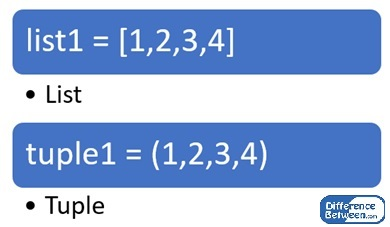
\includegraphics{Difference-Between-List-and-Tuple-fig-1-2.jpg}
\caption{At first glance list and tuples look very similar, but they are not\ldots{}}
\end{figure}

Like lists, tuples are containers of any type of object. Unlike lists though they are \emph{immutable} which means that once they have been created the content cannot be changed (i.e.~no append, insert or delete of the elements). Furthermore since they are immutable they can be used as dictionary keys (lists cannot).
To create a tuple the comma-separated list of items has to be enclosed in brackets, or the $\tt{tuple()}$ operator can be used.
Accessing tuple items is done in exactly the same way as lists.

\begin{tcolorbox}[breakable, size=fbox, boxrule=1pt, pad at break*=1mm, colback=cellbackground, colframe=cellborder]
\begin{Verbatim}[commandchars=\\\{\}]
\PY{n}{atuple} \PY{o}{=} \PY{p}{(}\PY{l+m+mi}{1}\PY{p}{,} \PY{l+m+mi}{2}\PY{p}{,} \PY{l+m+mi}{3}\PY{p}{)}
\PY{n+nb}{print} \PY{p}{(}\PY{l+s+s2}{\PYZdq{}}\PY{l+s+s2}{Length: }\PY{l+s+si}{\PYZob{}\PYZcb{}}\PY{l+s+s2}{\PYZdq{}}\PY{o}{.}\PY{n}{format}\PY{p}{(}\PY{n+nb}{len}\PY{p}{(}\PY{n}{atuple}\PY{p}{)}\PY{p}{)}\PY{p}{)}
\PY{n+nb}{print} \PY{p}{(}\PY{l+s+s2}{\PYZdq{}}\PY{l+s+s2}{First element: }\PY{l+s+si}{\PYZob{}\PYZcb{}}\PY{l+s+s2}{\PYZdq{}}\PY{o}{.}\PY{n}{format}\PY{p}{(}\PY{n}{atuple}\PY{p}{[}\PY{l+m+mi}{0}\PY{p}{]}\PY{p}{)}\PY{p}{)}
\PY{n+nb}{print} \PY{p}{(}\PY{l+s+s2}{\PYZdq{}}\PY{l+s+s2}{Last element: }\PY{l+s+si}{\PYZob{}\PYZcb{}}\PY{l+s+s2}{\PYZdq{}}\PY{o}{.}\PY{n}{format}\PY{p}{(}\PY{n}{atuple}\PY{p}{[}\PY{o}{\PYZhy{}}\PY{l+m+mi}{1}\PY{p}{]}\PY{p}{)}\PY{p}{)}

Length: 3
First element: 1
Last element: 3
\end{Verbatim}
\end{tcolorbox}

In the next snippet of code it is shown the so called unpacking which is another way to assign tuple values to variables.

\begin{tcolorbox}[breakable, size=fbox, boxrule=1pt, pad at break*=1mm, colback=cellbackground, colframe=cellborder]
\begin{Verbatim}[commandchars=\\\{\}]
\PY{n}{x}\PY{p}{,} \PY{n}{y}\PY{p}{,} \PY{n}{z} \PY{o}{=} \PY{p}{(}\PY{l+m+mi}{10}\PY{p}{,} \PY{l+m+mi}{5}\PY{p}{,} \PY{l+m+mi}{12}\PY{p}{)}
\PY{n+nb}{print} \PY{p}{(}\PY{l+s+s2}{\PYZdq{}}\PY{l+s+s2}{coord: x=}\PY{l+s+si}{\PYZob{}\PYZcb{}}\PY{l+s+s2}{ y=}\PY{l+s+si}{\PYZob{}\PYZcb{}}\PY{l+s+s2}{ z=}\PY{l+s+si}{\PYZob{}\PYZcb{}}\PY{l+s+s2}{\PYZdq{}}\PY{o}{.}\PY{n}{format}\PY{p}{(}\PY{n}{x}\PY{p}{,} \PY{n}{y}\PY{p}{,} \PY{n}{z}\PY{p}{)}\PY{p}{)}

coord: x=10 y=5 z=12
\end{Verbatim}
\end{tcolorbox}

If and ntuple has just one element don't forget the comma at the end otherwise it will be treated as a single number.

\begin{tcolorbox}[breakable, size=fbox, boxrule=1pt, pad at break*=1mm, colback=cellbackground, colframe=cellborder]
\begin{Verbatim}[commandchars=\\\{\}]
\PY{n}{tuple2} \PY{o}{=} \PY{p}{(}\PY{l+m+mi}{1}\PY{p}{,}\PY{p}{)}
\PY{n+nb}{print}\PY{p}{(}\PY{n+nb}{type}\PY{p}{(}\PY{n}{tuple2}\PY{p}{)}\PY{p}{)}
\PY{n}{tuple2} \PY{o}{=} \PY{p}{(}\PY{l+m+mi}{1}\PY{p}{)}
\PY{n+nb}{print}\PY{p}{(}\PY{n+nb}{type}\PY{p}{(}\PY{n}{tuple2}\PY{p}{)}\PY{p}{)}

<class 'tuple'>
<class 'int'>
\end{Verbatim}
\end{tcolorbox}

Since a tuple is immutable to add new elements it is necessary to create a new object:

\begin{tcolorbox}[breakable, size=fbox, boxrule=1pt, pad at break*=1mm, colback=cellbackground, colframe=cellborder]\begin{Verbatim}[commandchars=\\\{\}]
\PY{n}{tuple1} \PY{o}{=} \PY{p}{(}\PY{l+m+mi}{1}\PY{p}{,} \PY{l+m+mi}{2}\PY{p}{,} \PY{l+m+mi}{3}\PY{p}{)}
\PY{n}{tuple2} \PY{o}{=} \PY{n}{tuple1} \PY{o}{+} \PY{p}{(}\PY{l+m+mi}{4}\PY{p}{,} \PY{l+m+mi}{5}\PY{p}{)}
\PY{n+nb}{print}\PY{p}{(}\PY{n}{tuple2}\PY{p}{)}

(1,2,3,4,5)
\end{Verbatim}
\end{tcolorbox}

Finally, as already said tuples can be used as dictionary keys:

\begin{tcolorbox}[breakable, size=fbox, boxrule=1pt, pad at break*=1mm, colback=cellbackground, colframe=cellborder]\begin{Verbatim}[commandchars=\\\{\}]
\PY{n}{d} \PY{o}{=} \PY{p}{\PYZob{}}
   \PY{p}{(}\PY{l+s+s1}{\PYZsq{}}\PY{l+s+s1}{Finance}\PY{l+s+s1}{\PYZsq{}}\PY{p}{,} \PY{l+m+mi}{1}\PY{p}{)}\PY{p}{:} \PY{l+s+s1}{\PYZsq{}}\PY{l+s+s1}{Room 8}\PY{l+s+s1}{\PYZsq{}}\PY{p}{,}
    \PY{p}{(}\PY{l+s+s1}{\PYZsq{}}\PY{l+s+s1}{Finance}\PY{l+s+s1}{\PYZsq{}}\PY{p}{,} \PY{l+m+mi}{2}\PY{p}{)}\PY{p}{:} \PY{l+s+s1}{\PYZsq{}}\PY{l+s+s1}{Room 3}\PY{l+s+s1}{\PYZsq{}}\PY{p}{,}
    \PY{p}{(}\PY{l+s+s1}{\PYZsq{}}\PY{l+s+s1}{Math}\PY{l+s+s1}{\PYZsq{}}\PY{p}{,} \PY{l+m+mi}{1}\PY{p}{)}\PY{p}{:} \PY{l+s+s1}{\PYZsq{}}\PY{l+s+s1}{Room 6}\PY{l+s+s1}{\PYZsq{}}\PY{p}{,}
    \PY{p}{(}\PY{l+s+s1}{\PYZsq{}}\PY{l+s+s1}{Programming}\PY{l+s+s1}{\PYZsq{}}\PY{p}{,} \PY{l+m+mi}{1}\PY{p}{)}\PY{p}{:} \PY{l+s+s1}{\PYZsq{}}\PY{l+s+s1}{IT room}\PY{l+s+s1}{\PYZsq{}}
    \PY{p}{\PYZcb{}}
\end{Verbatim}
\end{tcolorbox}

Below the full list of tuple functions:
\begin{tcolorbox}[breakable, size=fbox, boxrule=1pt, pad at break*=1mm,colback=cellbackground, colframe=cellborder]
\begin{Verbatim}[commandchars=\\\{\}]
\PY{n+nb}{dir}\PY{p}{(}\PY{n+nb}{dict}\PY{p}{)}

[...
 'count',
 'index']
\end{Verbatim}
\end{tcolorbox}
